\documentclass{article}

\usepackage[final]{neurips_2023}

\usepackage[utf8]{inputenc}
\usepackage[T1]{fontenc}
\usepackage{hyperref}
\usepackage{url}
\usepackage{booktabs}
\usepackage{amsfonts}
\usepackage{amsmath}
\usepackage{nicefrac}
\usepackage{microtype}
\usepackage{xcolor}
\usepackage{graphicx}
\usepackage{subcaption}
\usepackage{wrapfig}
\usepackage{titlesec}
\usepackage{needspace}

\setlength{\tabcolsep}{6pt}
\renewcommand{\arraystretch}{1.05}
\titlespacing*{\section}{0pt}{2.0ex plus 0.5ex minus 0.2ex}{0.9ex plus 0.2ex}
\titlespacing*{\subsection}{0pt}{1.2ex plus 0.3ex minus 0.1ex}{0.5ex plus 0.1ex}
\setlength{\textfloatsep}{8pt plus 2pt minus 2pt}
\setlength{\intextsep}{8pt plus 2pt minus 2pt}
\setlength{\abovecaptionskip}{4pt}
\setlength{\belowcaptionskip}{0pt}
\widowpenalty=10000
\clubpenalty=10000
\displaywidowpenalty=10000
\raggedbottom

\title{MLPC 2026 Task 4: Data Classification Report}

\author{%
  Team A-C (Qualitative) \AND
  Julian Schmidt, Paul Breburda
}

\begin{document}

\maketitle

We train and evaluate segment-level multi-label classifiers for the KIAL domestic sound event dataset. Building on the Task 3 analysis, we convert the $[T,C,A]$ annotator overlap tensors into binary labels, build leakage-controlled train/validation/test splits, normalize and contextualize the 960-dimensional audio features, and compare a linear classifier against neural networks. The final logistic regression reaches 0.529 test macro AP, while a validation-selected MLP ensemble reaches 0.638 test macro AP and 0.754 test micro AP, a tenfold improvement over the class-prior baseline in macro AP.

\section{Dataset Preparation}

\subsection{Label Aggregation}

Each feature file contains an annotation tensor $\mathrm{ann}\in[0,1]^{T\times C\times A}$ with one-second segments, 15 classes, and a variable number of annotators. We drop annotator slices with no finite nonzero information, binarize each remaining annotator's overlap at 0.5, and take a strict majority vote over annotators for segment $t$ and class $c$:
% NOTE (label rule): outer threshold is strict (> 0.5) so that a 1-of-2 vote does NOT
% produce a positive, matching the prose ("events marked by only one annotator vanish").
% The actual majority_vote() implementation was NOT provided with this report and could
% not be inspected; verify the code uses a strict ">" before final submission.
\[
y_{t,c}=\mathbf{1}\!\left[
\frac{1}{A}\sum_{a=1}^{A}\mathbf{1}[\mathrm{ann}_{t,c,a}\geq 0.5] > 0.5
\right].
\]
This maps $[T,C,A]$ to $[T,C]$ and matches the segment-level objective: a segment is positive only when at least half of it is covered by an event and a strict majority of valid annotators agree. The advantage over a union rule is precision; Task 3 showed missed and confused labels on polyphonic clips, so accepting every single-annotator event would inject many false positives. The cost is recall: with two annotators, an event marked by only one vanishes, which especially hurts brief classes such as \texttt{light\_switch}.

\subsection{Leakage-Controlled Split}

\begin{wrapfigure}{r}{0.46\linewidth}
  \centering
  \vspace{-1.2em}
  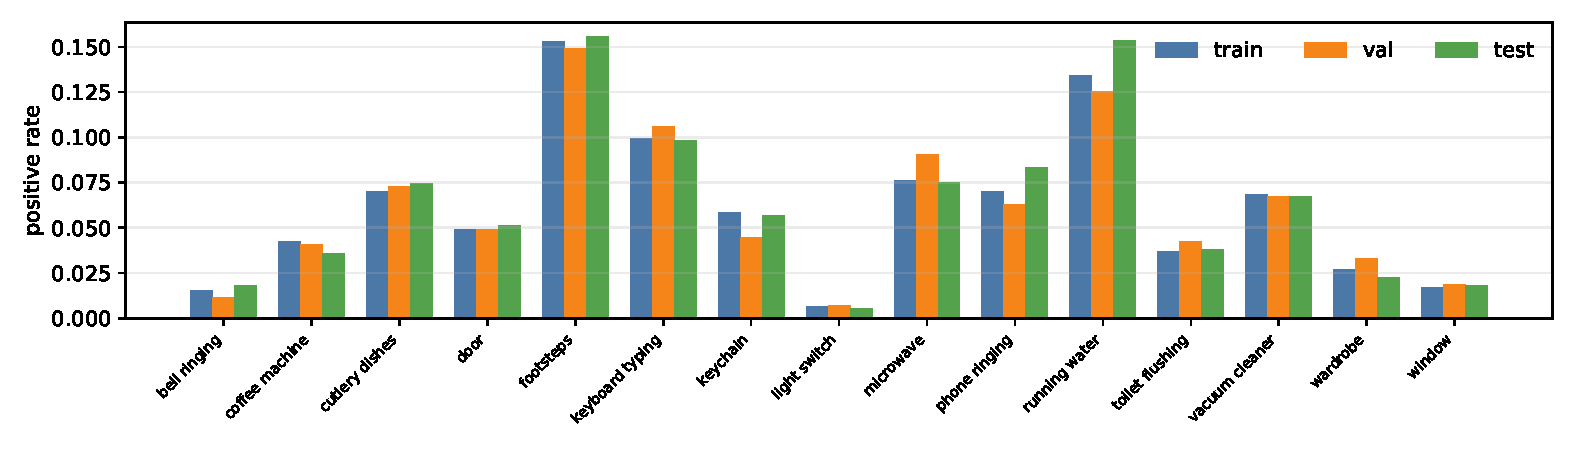
\includegraphics[width=\linewidth]{figures/class_dist_across_splits.pdf}
  \caption{Positive segment rates per class after the collector-disjoint split.}
  \label{fig:splits}
  \vspace{-1.0em}
\end{wrapfigure}

The split is collector-disjoint, not segment- or file-random. We use grouped random splitting with 70\%/15\%/15\% target proportions, yielding 116{,}950 train segments from 2{,}553 files and 285 collectors, 25{,}733 validation segments from 548 files and 61 collectors, and 25{,}556 test segments from 555 files and 62 collectors. This prevents three leakage modes: adjacent segments from the same recording sharing background noise, recordings from the same collector sharing rooms and devices, and hyperparameters being tuned on the same distribution used for final reporting. Segments from the same recording and recordings from the same collector therefore never appear in multiple splits.

Class distributions should stay similar because macro AP weights rare and frequent classes equally. Exact stratification is impossible under collector grouping, but Figure~\ref{fig:splits} shows the split preserves the main prevalence pattern: \texttt{footsteps} and \texttt{running\_water} stay common while \texttt{light\_switch}, \texttt{bell\_ringing}, and \texttt{window\_open\_close} stay rare. Small deviations, e.g.\ \texttt{microwave} being more common in validation, are the price of avoiding leakage.

\subsection{Preprocessing}

We concatenate all 56 aggregated feature arrays from the 14 acoustic groups into a 960-dimensional vector. A standard scaler is fit on training segments only and applied to validation and test, since spectral centroid, power, mel bands, flatness, and MFCC-derived features differ widely in scale; without z-scoring, linear models and neural optimization are dominated by high-variance features. The final models add temporal context by concatenating the two preceding and two following segments from the same recording, with zero padding at file boundaries. This yields 4{,}800 input dimensions and lets the classifier exploit onset/offset evidence spread across the 0.5\,s hop grid.

\section{Evaluation}

\subsection{Metric}

We select models by validation macro average precision (macro AP). AP is threshold-free, evaluating the probability ranking directly rather than relying on an arbitrary 0.5 decision threshold. Macro averaging is essential here because \texttt{footsteps} has 25{,}685 positive segments while \texttt{light\_switch} has only 1{,}047; micro AP would mainly reward common, sustained events. We still report micro AP to describe overall segment-ranking quality.

\subsection{Baseline and Performance Ceiling}

The baseline predicts each class's empirical training prevalence for every segment. With no access to audio features it obtains 0.0636 test macro AP and 0.1207 test micro AP (Table~\ref{tab:final}). A perfect AP of 1.0 is the formal maximum, but the realistic ceiling is lower: Task 3 measured only moderate annotator agreement, and the weakest classes are exactly those with ambiguous boundaries or acoustic confusions, such as \texttt{light\_switch}, \texttt{door\_open\_close}, and \texttt{wardrobe\_drawer\_open\_close}.

\begin{table}[t]
  \centering
  \small
  \caption{Validation-selected models evaluated on the held-out test split.}
  \label{tab:final}
  \begin{tabular}{lccc}
    \toprule
    Model & Val. Macro AP & Test Macro AP & Test Micro AP \\
    \midrule
    Class prior & 0.0615 & 0.0636 & 0.1207 \\
    Logistic regression & 0.4936 & 0.5287 & 0.6637 \\
    MLP ensemble & 0.6178 & 0.6381 & 0.7544 \\
    \bottomrule
  \end{tabular}
\end{table}

\section{Experiments}

\subsection{Logistic Regression}

The first model is a one-vs-rest linear logistic classifier with independent sigmoid heads, trained with AdamW on the normalized temporal-context features. We varied four hyperparameters: feature representation (single segment vs.\ context), learning rate, weight decay, and positive-class weighting. Context was decisive: non-context runs stayed near 0.45 validation macro AP while context runs reached 0.49. The top validation setting used context features and learning rate $3\cdot10^{-3}$, with weight decay $10^{-4}$ and positive weights clipped at 10. Stronger class weighting improved rare-class recall but lowered ranking quality on common classes; no weighting improved micro AP but hurt macro AP.
% NOTE: Figure 2 (validation-AP settings bar charts, figures/hyperparameter_summary.pdf) was
% removed to meet the 3-page limit; its content is summarized in the sentence above. With that
% figure gone, no settings/bar plot remains, so the "pw=nan -> pw=none" relabel and the
% duplicate-bar disambiguation in instruction 4 are not applicable here.

\subsection{MLP and Ensembling}

The second model is a feed-forward network with ReLU activations, dropout, AdamW, and class-weighted binary cross-entropy. We varied width/depth, dropout, learning rate, seed, and training duration. The best single checkpoint used hidden layers $[512,256]$, dropout 0.45, learning rate $10^{-3}$, and early stopping after 43 epochs, reaching 0.599 validation macro AP; wider networks such as $[1024,512]$ were close but less consistent. Because several strong checkpoints made complementary ranking errors, we averaged their predicted probabilities. A greedy eight-checkpoint ensemble raised validation macro AP to 0.618 and was selected as the final MLP.

\subsection{Model Comparison}

\begin{wrapfigure}{r}{0.50\linewidth}
  \centering
  \vspace{-1.1em}
  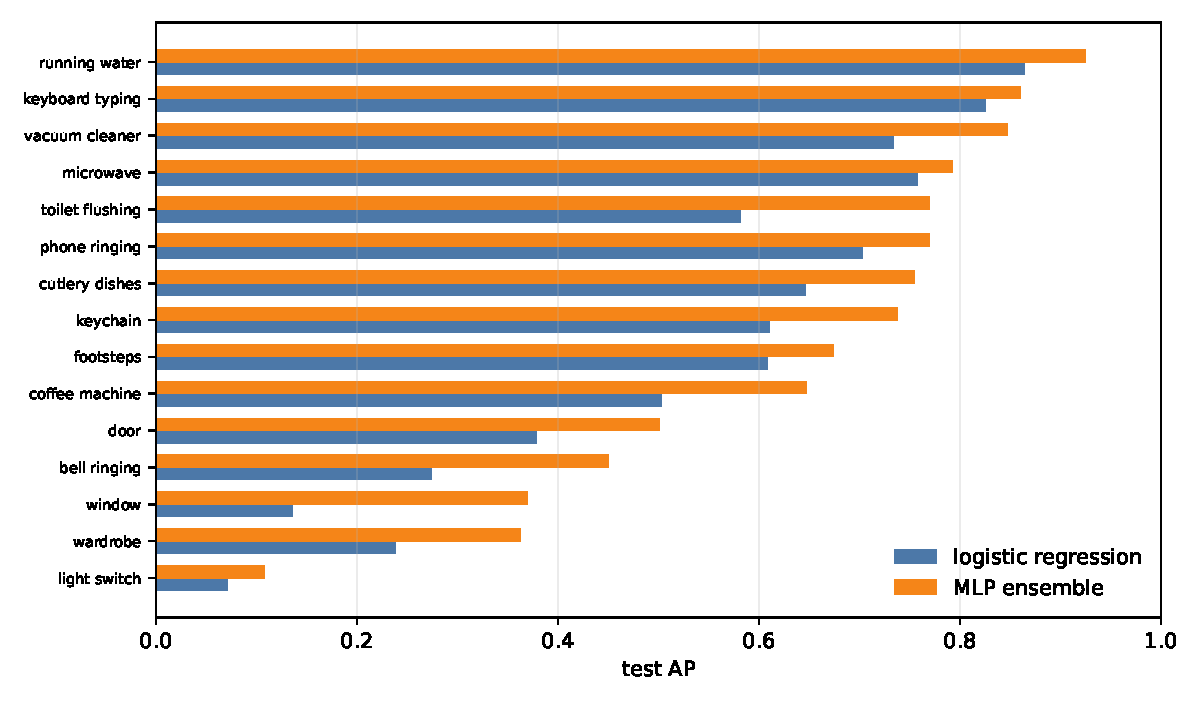
\includegraphics[width=\linewidth]{figures/per_class_ap.pdf}
  \caption{Per-class test AP for the two learned classifiers, sorted by MLP performance.}
  \label{fig:perclass}
  \vspace{-1.0em}
\end{wrapfigure}

Both classifiers far outperform the baseline, but the MLP is stronger on every aggregate metric (Figure~\ref{fig:perclass}). Logistic regression already separates sustained sounds well, showing the precomputed features are informative and that temporal context matters. The MLP adds nonlinear feature interactions and lifts the difficult middle range: \texttt{toilet\_flushing} rises from 0.581 to 0.770 AP, \texttt{window\_open\_close} from 0.135 to 0.370, and \texttt{bell\_ringing} from 0.274 to 0.450. The remaining gap is concentrated in rare transients and mechanically similar events.

\section{Case Study and Reflection}

\subsection{Qualitative Test Files}

We selected two held-out recordings using the final MLP probabilities and majority-vote labels (Table~\ref{tab:cases}, Figure~\ref{fig:cases}). File 000727 is a successful kitchen recording whose metadata describes starting a microwave, running water, and washing dishes; the model tracks all three active classes and reaches file-level F1 0.978 at threshold 0.5. File 000892 is a failure case from a mobile hallway recording with a door opening, footsteps, a light switch, and a coat hanger: the model fires, but not on the correct class--time pairs, yielding F1 0.000.

\begin{table}[t]
  \centering
  \small
  \caption{Held-out qualitative cases for the final MLP.}
  \label{tab:cases}
  \begin{tabular}{llcc}
    \toprule
    File & Active classes & Segments & F1 \\
    \midrule
    000727 & \texttt{cutlery}, \texttt{microwave}, \texttt{running\_water} & 47 & 0.978 \\
    000892 & \texttt{door\_open\_close}, \texttt{footsteps}, \texttt{light\_switch} & 45 & 0.000 \\
    \bottomrule
  \end{tabular}
\end{table}

\begin{figure}[t]
  \centering
  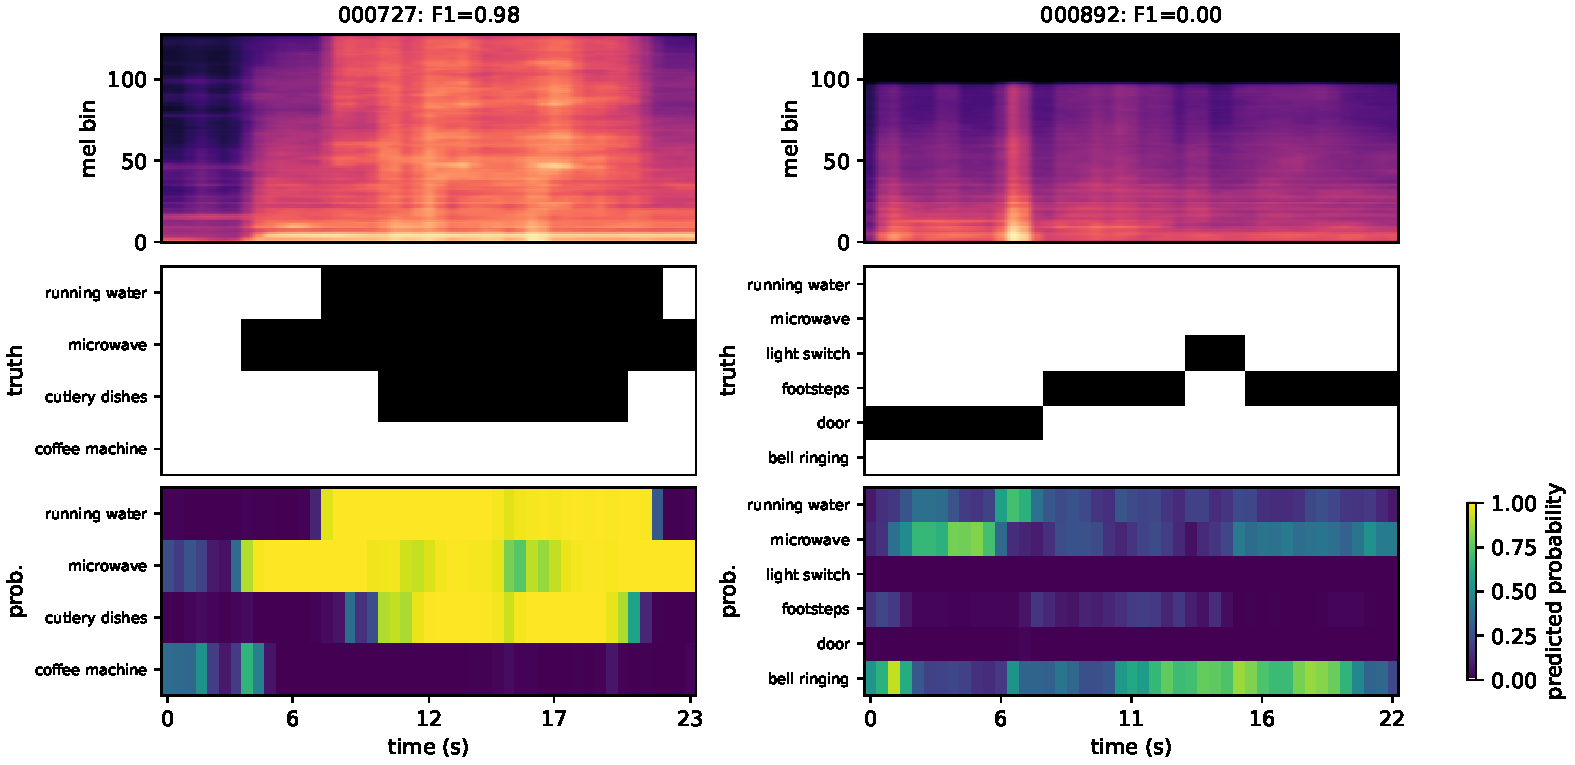
\includegraphics[width=0.92\linewidth,height=5.0cm,keepaspectratio]{figures/case_studies.pdf}
  \caption{Case studies on non-training files (000727, left; 000892, right). Top: provided mel-spectrogram features; middle: majority-vote labels; bottom: MLP probabilities.}
  \label{fig:cases}
\end{figure}

\subsection{Strengths and Failure Modes}

The final model is reliable for sustained or spectrally distinctive events: \texttt{running\_water} (0.925 AP), \texttt{keyboard\_typing} (0.861), \texttt{vacuum\_cleaner} (0.847), and \texttt{microwave} (0.793). These produce long, repeated evidence across adjacent segments, so the context window and AP-based objective work well. The weakest classes are \texttt{light\_switch} (0.108), \texttt{wardrobe\_drawer\_open\_close} (0.363), \texttt{window\_open\_close} (0.370), and \texttt{bell\_ringing} (0.450). Their errors follow three patterns: short transients are missed or shifted by one segment; door/window/wardrobe actions are confused because they share mechanical impact and hinge sounds; and rare classes carry too little positive evidence for stable ranking. A raw-audio temporal model, focal loss, or post-processing with event-duration priors is the most promising next step, but the current MLP already provides a robust feature-based detector for the development set.

\section{Disclosure of LLM and AI Tool Use}

We used GPT-5.5 and Claude Opus 4.8 through a local coding agent for experiment orchestration, code generation, result summarization, figure generation, and editorial refinement of this report. All quantitative claims were verified by rerunning the Python pipeline and cross-checking the produced artifacts: \texttt{results/final\_table.csv}, \texttt{results/lr\_torch\_sweep.csv}, \texttt{results/mlp\_sweep.csv}, and \texttt{results/mlp\_ensemble\_sweep.csv}. Figures were produced programmatically from the same dataset and prediction files and inspected for consistency with the reported metrics. The entire Code for this Assignment is available here \href{https://github.com/Julian-AT/mlpc_task_4}{available here}

\end{document}